%! TEX root = ../main.tex
\chapter{研究设计}\label{chap:3}
\section{极端天气的范围选择}\label{sec:def}

在气候变化的大背景下,异常气候以及极端天气事件发生的可能性增加\citep{aigner2023summary,donat2017addendum},这其中极端强降水愈发频繁\citep{trenberth2010relationships}。气候代表了一个地区在一定时间跨度内所经历的天气状况的总体特征,揭示了一个地区的基本气象冷热、干湿特性,故而温度和降水是构成某一地区气候特征的两个最根本的气象要素\citep{alexander2006global}。在我国,极端天气事件如洪涝、干旱、台风、暴雪等自然灾害\citep{尹红2019基于},往往与极端强降水事件密切相关,给国家和人民带来了巨大的损失。因此,本文选取将极端降水作为极端天气事件的代表来进行深入分析。

对于极端降雨强度的定义,国家标准 GB/T 33680-2017《暴雨灾害等级》中将日降水量超过 50mm 定义为暴雨,超过 250mm 定义为特大暴雨。然而,由于不同地区在气候特征和降水模式上存在显著差异,单一的数值标准可能无法全面反映极端降水事件的影响。参考国际气候变化检测和指数专家组(ETCCDI)采用分位数来定义极端天气的方法,将日降水量超过95th或99th百分位数的情况定义为极端降水,这种方法能够更好地适应不同地区的降水特征,因此本文选择将极端降水天气定义为20年一遇的降水天气。

而关于极端降雨受灾范围的界定,结合降水数据和保单数据(见\ref{sec:data}),考虑到绝大多数保险标的与距离最近的气象站之间距离大多在50公里以内,平均距离不足30公里,如图\ref{fig:distance},因此本文将距离监测到极端降水的气象站20公里内的区域定义为灾区。而考虑到我国气象站分布间距基本在100公里以内,如图\ref{fig:locations},因此取气象站所覆盖的受灾半径最多为50公里,定义距离监测到极端降水的气象站20-50公里内的区域为近灾区,50公里以上的区域为远灾区。

\begin{figure}[H]
    \begin{minipage}{0.48\linewidth}
        \centering
        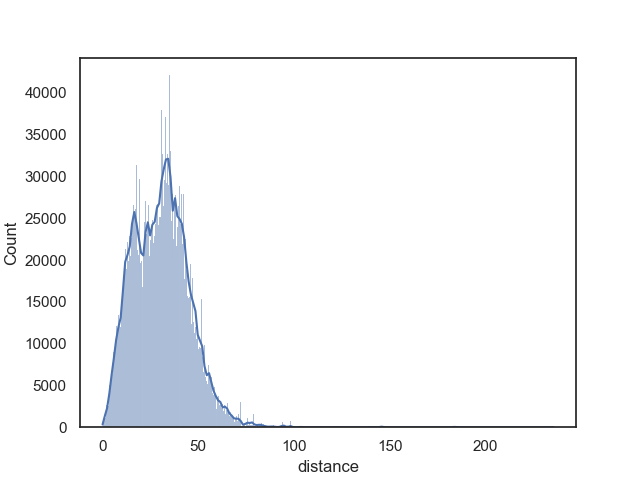
\includegraphics[width=\textwidth]{lib/img/distance.png}
        \caption{原始数据中保险标与最临近气象站的距离分布(千米)}
        \label{fig:distance}
    \end{minipage}
    \begin{minipage}{0.48\linewidth}
        \centering
        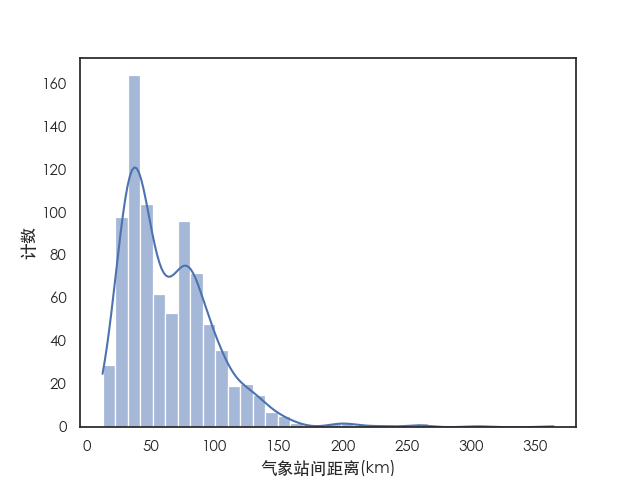
\includegraphics[width=\textwidth]{lib/img/locations_distance.png}
        \caption{原始数据中气象站间距的地理位置分布(千米)}
        \label{fig:locations}
    \end{minipage}
\end{figure}

\section{样本选择与数据来源}\label{sec:data}

本文选取了中国气象局的气象数据和某财产保险公司的承保理赔保险数据作为研究数据。空间范围上,二者均覆盖全国。大多数研究在数据预处理时通常聚类至县市一级行政区划\citep{0Do,杨娜娜2019自然灾害与企业现金持有},得益于GIS技术的发展和普及化,本文对于数据的处理相较于更为精细,直接根据经纬度信息计算距离,不再依赖行政区划的聚类,从而提高了数据的空间精度,也更符合我国地理环境的多样性和复杂性。。时间维度上,气象数据时间范围为1954年1月1日至2015年12月31日,保险数据时间范围为1995年1月1日至2019年12月31日,数据清洗时保留1995-2015年数据。

% TODO:比例尺
\begin{figure}[H]
    \centering
    \begin{minipage}{0.48\linewidth}
        \includegraphics[width=\textwidth, trim=200 0 200 0]{lib/img/locations.png}
        \caption{原始数据中气象站的地理位置分布}
        \label{fig:location}
    \end{minipage}
    \begin{minipage}{0.48\linewidth}
        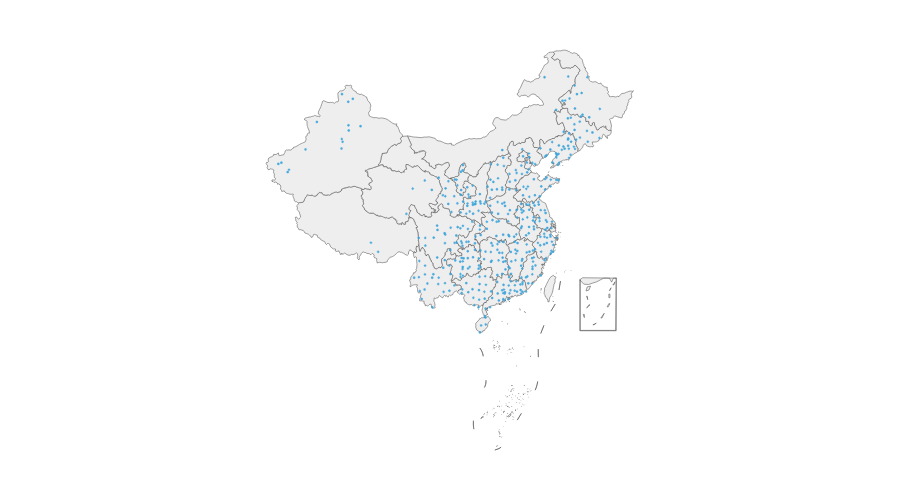
\includegraphics[width=\textwidth, trim=200 0 200 0]{lib/img/near.png}
        \caption{划分为灾区气象站的地理位置分布}
    \end{minipage}
\end{figure}
\begin{figure}[H]
    \begin{minipage}{0.48\linewidth}
        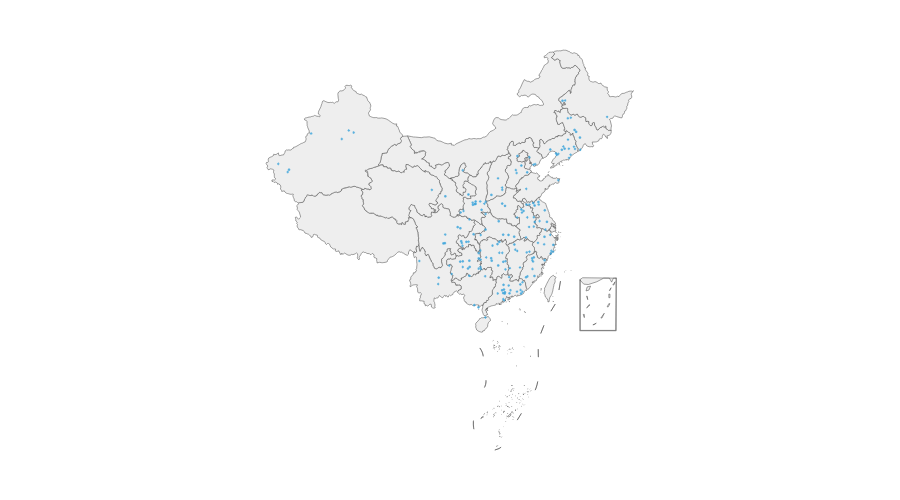
\includegraphics[width=\textwidth, trim=200 0 200 0]{lib/img/middle.png}
        \caption{划分为近灾区气象站的地理位置分布}
    \end{minipage}
    \begin{minipage}{0.48\linewidth}
        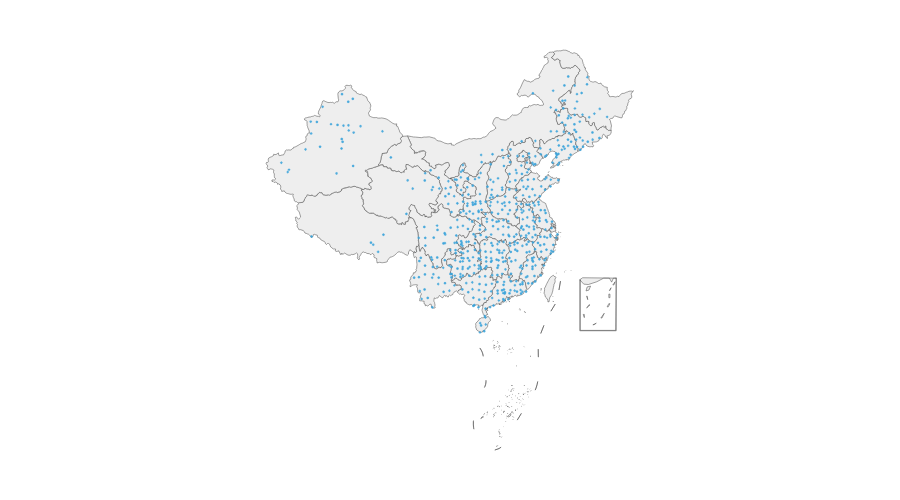
\includegraphics[width=\textwidth, trim=200 0 200 0]{lib/img/far.png}
        \caption{划分为非灾区气象站的地理位置分布}
    \end{minipage}
\end{figure}
进一步的数据处理流程包括:首先,我们对连续变量进行了缩尾处理,即在数据的首尾1\%处进行了截断。其次,为了确保气象数据与保单数据之间的相关性,我们对选取的保单进行了地理限制,只选择了那些距离最近的监测站20公里以内的保单进行分析。这样的限制有助于确保气象数据与保单之间的相关性更加紧密,因为气象条件对保险赔付的影响往往与地理位置密切相关。

在完成了上述数据处理步骤后,本文最终将1914万条气象数据与610万条保单数据进行了匹配,得到约了70万条可用于回归分析的数据。

\section{模型设定与变量选取}

极端天气事件是一个外生冲击,在时空上的分布是随机的,因此本文采用了DID回归来估计极端天气事件对家庭财产保险的影响。DID回归的基本思想是通过对照组和实验组的比较,消除了时间不变的个体特征对估计结果的影响,从而更加准确地估计政策的效果。本文设定了一个虚拟的实验组和对照组,实验组为受灾区或近灾区,对照组为未受灾区,通过比较两组在巨灾发生前后的差异来估计极端天气事件对财产保险的影响。

本文采用的主要被解释变量为家财险保额,反映家庭对财产保险的需求。而主要解释变量为极端天气事件的虚拟变量,分为两个维度:一是是否受灾,即家庭所在地区是否直接遭受了极端天气事件的影响;二是是否邻近灾区,即使家庭所在地区未直接受灾,但若邻近地区遭受灾害,也可能会影响他们的保险需求。

\begin{figure}[H]
    \begin{minipage}{0.48\linewidth}
        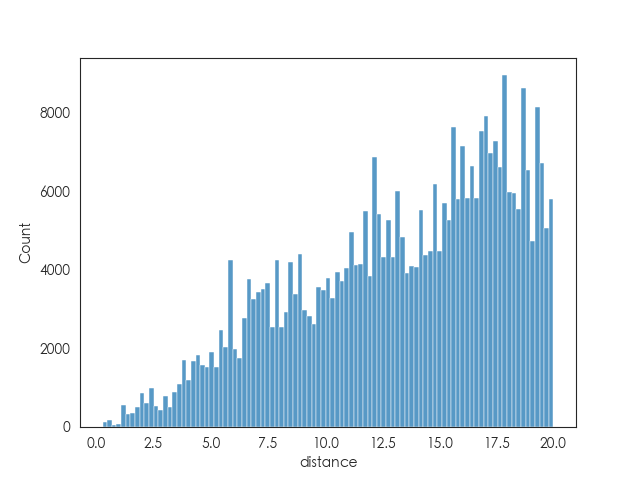
\includegraphics[width=\linewidth]{lib/img/olsdistance.png}
        \caption{回归中标的与监测站距离分布}
    \end{minipage}
    \begin{minipage}{0.48\linewidth}
        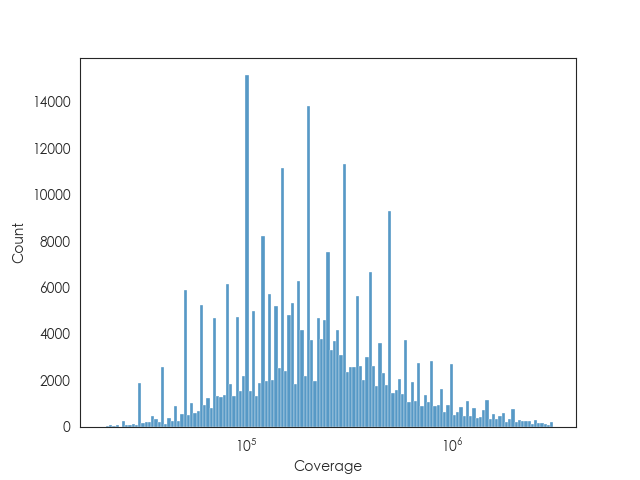
\includegraphics[width=\linewidth]{lib/img/coverage.png}
        \caption{回归中标的保额对数分布}
    \end{minipage}
\end{figure}

此外,为了更全面地评估极端天气事件的影响,本文纳入一系列控制变量。这些变量包括:
\begin{enumerate}
    \item 是否历史投保:反映了家庭过去的保险购买行为,可能影响他们对未来保险需求的决策。
    \item 保险财产购置价:反映了家庭财产的价值,通常财产价值越高,保险需求也越大。
    \item 建筑面积:建筑面积越大,需要更高的保险保额来覆盖潜在的风险。
\end{enumerate}
\begin{table}[H]
    \caption{变量定义表}\label{tab:var}
    \centering
    \begin{tabular}{@{}cccc@{}}
        \toprule
        变量类别                    & 变量名称         & 变量定义    & 变量解释                \\ \midrule
        被解释变量                   & Coverage     & 保额      & 保险金额                \\ \midrule
        \multirow{3}{*}{主要解释变量} & Disaster     & 灾区      & 是否处于极端降水监测点20公里内    \\ \cmidrule(l){2-4}
                                & Neighbor     & 近灾区     & 是否处于极端降水监测点20-50公里内 \\ \cmidrule(l){2-4}
                                & Post         & 降水发生时间  & 是否在极端降水发生后投保        \\
        \midrule
        \multirow{3}{*}{控制变量}   & Prem\_before & 历史投保    & 保险标的是否有投保记录         \\ \cmidrule(l){2-4}
                                & Price        & 保险财产购置价 & 保险标的资产购置价           \\ \cmidrule(l){2-4}
                                & Area         & 建筑面积    & 保险标的建筑面积            \\ %\cmidrule(l){2-4}
        % & Claim       & 是否理赔    & 该保单是否发生理赔            \\
        \bottomrule
    \end{tabular}
\end{table}


考虑保额分布有下界,不满足正态分布,因此针对假设H\ref{hyp:1}、假设H\ref{hyp:2}本文的DID模型如下:

\begin{equation}
    \log\text{Coverage}=\alpha+\beta_1\text{Disaster}+\beta_2\text{Post}+\beta_3\text{Disaster}\times\text{Post}+\beta\text{Controls}+\varepsilon
    \label{eq:DID_1}
\end{equation}

而针对假设H\ref{hyp:3}本文的DID模型如下:

\begin{equation}
    \log\text{Coverage}=\alpha+\beta_1\text{Neighbor}+\beta_2\text{Post}+\beta_3\text{Neighbor}\times\text{Post}+\beta\text{Controls}+\varepsilon
    \label{eq:DID_2}
\end{equation}


